
\section*{Satisfiability Modulo Theories and Automated Theorem Proving:\\ Quest for the Missing Link}

\vspace{-.5em}
\hrule

\vspace{1.2em}
Beginning with the 1980's, the computer science community has accepted
that computer programs and logical proofs are made of the same fabric.
They are both based on a rigorous formal language, characterized by a grammar,
and they both rely heavily on tree-like structures for defining their semantics,
via syntax-directed derivations.
By now, it has become widely accepted~\cite{curry-howard} that the task of writing a program can be
reduced to that of finding a proof to a conjecture, and conversely, the task of
proving a theorem can be reduced to producing a program with some specific
characteristics.
In addition to that, logic is at the core of software verification, as a basis
for specifications~\cite{dafny,boogie,seahorn}, loop invariants~\cite{ic3,spacer,..}, rely-guarantee properties~\cite{relyguarantee1,..}, and more.
The task of checking adherence to a program's specification is also reduced, in
more than one way, to deciding the validity of a logical formula.

\medskip
This proposal is based on a fundamental understanding, that breaking existing
barriers in automated reasoning is a key ingredient that will lead to
much more powerful mechanism for the construction of provably-correct software.
By powerful, we mean scalable to the sizes of realistic software modules,
adaptable to arbitrarily complex properties,
and requiring less user effort thanks to an increased level of automation.
To achieve this goal, this research \textbf{aims to bridge the gap between two insofar prevalent automated  reasoning disciplines}:

\begin{paragraph}{Automated Theorem Provers (ATP)} A family of tools and techniques based on proof
theory of logical deduction.
A logic in this setting is characterized by a vocabulary and a system of
inference rules; provers are tasked with searching the space of proofs, which
are essentially trees (more generally, DAGs) constructed from repeated
application of the inference rules.
\end{paragraph}

\begin{paragraph}{Satisfiability-Modulo-Theory Solvers (SMT)} A somewhat newer approach with roots in complexity theory and algorithms for solving the Boolean satisfiability problem (SAT).
These algorithms have been augmented with decision procedures for several first-order fragments.
SMT solvers have become incredibly popular thanks to highly efficient implementations and very successful optimization heuristics that manage to combat the inherent intractability of the problem.
\end{paragraph}

\medskip

%\todo{Merge description of ATP and SMT to the background; write here a short paragraph defining these two things and saying that the idea is to merge them}


%The expected result is a proof leading to a desired statement (closed formula)
%$\varphi$, that can be used as a certificate to the logical validity of
%$\varphi$ --- that is, it can be checked mechanically to confirm the soundness
%of each inference step.
%While proof search can be a very costly process, due to the inherent complexity
%of the search space, checking a proof is usually swift and done with linear
%cost with respect to its size.

\begin{comment}

%\begin{comment}
\todo{remove this from here and put in background, it kills the flow}
It is worth mentioning a third camp, that has, so far, received less
attention from the programming languages and automated reasoning crowd.

\paragraph{CSP Solvers} Constraint Satisfaction Problems (CSP) are ubiquitous
in planning, AI, and various other fields of computer science.
The ultimate goal of CSP is to find parameters that satisfy a set of (mostly
numerical) constraints. The solutions can be useful for scheduling tasks,
motion planning, \etc.
CSP solvers excel at solving puzzles such as the $N$-queen problem or Sudoku.
Their use in automated theorem proving is insofar limited.
\end{comment}

\medskip
These two camps, coming from such different backgrounds,
face a serious gap,
one that currently prevents adoption of results from one approach into use in
the other.
The primary goal of this research is to construct a unified framework for automated reasoning, where proving
and solving techniques can cooperate.
Such framework need not be constrained by the boundaries of some specific logic, such as first-order logic or linear integer arithmetic.
Instead, careful parameterization will allow adaptive treatment of a wide spectrum of domains, where existing techniques can be seen as individual points in the more general space.
This will allow to leverage the power of ATP and SMT into proving the more complex
conjectures required for software verification and synthesis.
When it comes to applying SMT, one major obstacle in many problem domains, is
that SMT solvers are generally restricted to first-order logic; at the same time,
the properties one wishes to prove require reasoning about composite structures (such as lists, maps, and streams), and, most often, the use of induction.
Theorem provers can more easily be equipped with higher-order logic and induction-oriented inference
rules.
Still, sub-problems arising in the course of resolving the induction step can
and should benefit from honed SAT and SMT capabilities.

As an overarching goal, this research will \textbf{lay foundations for a new discipline
in automated provers, by way of integrating the camps of ATP and SMT and allowing
cross-fertilization}.
Specifically, it is motivated by provers for the tasks of software verification
and synthesis; these are characterized by relying almost exclusively on discrete
mathematics, such as set theory, graphs, automata, an algebraic construction of
natural numbers, and various theories of integer arithmetic.


\section{Background}

\todo{The background should put an emphasis on what each tool is good at}

\begin{paragraph}{Automated Theorem Provers}
Proof theory is a branch of logic that has gained much traction in the 20th century with the advent of Hilbert~\cite{Book1928:Hilbert} and Gentzen~\cite{j1935:Gentzen},
both of whom developed calcli for algorithmic formalization of proofs.
As computers became available, it was natural that these notions be implemented as programs.
As early as 1960~\cite{otter}, large automatic systems for theorem provers have been used by the research community for a variety of logical reasoning tasks.
Most of these early systems were based on the resolution principle~\cite{robinson1965}, which continues to be popular today.
Term unification~\cite{robinson1965} is used to resolve first-order formulas.
In the 1990's, superposition calculus~\cite{LPAR1992:Bachmair} emerged as the leading technique for equality reasoning.
This led to several successful theorem provers, notably Vampire~\cite{JAR1995:Voronkov} and E prover~\cite{AIC2002:Schulz}.
Today, most theorem provers rely in one way or another on term rewriting for the implementation of superposition, based on the Knuth-Bendix algorithm~\cite{knuth-bendix} for normalizing rewrites.

More recently, a lot of attention was directed towards \emph{cyclic proof systems}, a form of Gentzen-style calculus that natively admits proof by induction.
Instead of the traditional induction scheme or induction rule, \eg (for $\mathbb{N}$) $P(0)\land \forall k.\,P(k)\to P(k+1) \vdash \forall n.\,P(n)$,
cyclic proofs admit ancestor sequents as premises to a later inference steps --- thereby allowing the proofs to contain cycles.
To avoid unsoundness caused by a self-referencing statement, cyclic proof systems impose a \emph{global trace condition} that ensure cycles cannot be unrolled \textit{ad infinitum}.
This trace condition is carefully crafted for every cyclic system to enable a soundness proof for the system.
In a way, whatever complexity is removed from the proof proper is shifted to the global trace condition;
however, this allows for some pretty sophisticated trace conditions, such as those based on B\"uchi automata.
In turn, these allow such systems to provide exetremely succinct and elegant proofs.
\end{paragraph}

\begin{paragraph}{Satisfiability-Modulo-Theory Solvers}
A somewhat newer approach based on extending the
Boolean satisfiability problem (SAT) with first-order theories and arithmetic, leading to
Satisfiability Modulo Theory (SMT).
SAT solvers accept Boolean formulas and construct a satisfying assignment, or
declare that none exists.
Since SAT is NP-complete (in fact, usually referred to as \emph{the} canonical
NP-complete problem), finding the solution may be time consuming, but eventual
termination is guaranteed.
SMT solvers take first-order formulas and attempt to find a first-order
\emph{model} for them, that is consistent with an underlying theory --- where the
theory is built into the solver.
The theories generally put no bound on the size of the models they admit
(\eg, numerical theories are typically defined over the domain of integers),
and as expected, the problem is generally undecidable.
However, despite the inherent complexity of SAT and undecidability of SMT,
solver technology has become extremely successful, especially in applications
relating to software verification.
In this context, proving a verification condition (``theorem'') $\varphi$
amounts to finding its negation $\lnot\varphi$ unsatisfiable --- which is the root
of the connection, and contention, between SMT solvers and theorem provers.
For many software verification conditions, SMT solvers have been shown to be
more effective in proving the validity of verification conditions than
contemporary proof theory-based theorem provers.

SAT and SMT received much tractions in the Model Checking community~\cite{clarke-grumberg} thanks to their successful applications to formal methods.
SAT was initially utilized for hardware verification of logical circuits, and SMT became a natural extension for dealing with software, as programming languages typically provide primitives such as integer values~\cite{CAV2006:Dutertre}, bit vectors~\cite{TACAS2007:Bryant}, and arrays~\cite{CAV2007:Ganesh}.
Because loops are pervasive in both hardware and software systems, there is an ever-present need for reasoning about executions of unbounded length.
To that end, \emph{loop invariants} play a crucial role in all software verification systems~\cite{dafny,fstar,leon}.
This essentially facilitates an induction scheme, but, by and large, the burden of supplying the invariant remains with the programmer.
\emph{Invariant inference} is a big open problem that stands in the way to effective software verification.
A significant breakthrough in invariant inference was achieved last decade with the development of the IC3 algorithm~\cite{bradley11} for automatic inference of Boolean invariants for hardware model checking.
This sprouted a line of successful follow-up works on Property-Directed Reachability~\cite{gurfinkel,shoham,vizel}.
These results have been integrated into the leading SMT solver Z3~\cite{z3,spacer} and form key components of the SeaHorn verifier~\cite{seahorn} for C programs.
\end{paragraph}


\section{Bridging the Automated Reasoning Gap}

\todo{Be more specific about the problems and why they are important: e.g. "cope with Boolean constructs", "unavoidable in software verification" etc.; explain what gives rise to these instances}

\begin{paragraph}{Objective 1: {\it Bridging induction}}~
The success of SMT solvers with first-order reasoning led to their wide adoption in software verification.
This gives rise to the challenge of representing unbounded state (\eg size of data structures) and unbounded time (\eg number of loop iterations).
The proposed framework will try to generalize and unify the two leading frontiers for reasoning by induction.
In the world of model checking and SMT, the IC3 algorithm and its variants~\todo{remember to cite them in the background} has proven to be the gold standard for automatic invariant inference.
In proof theory and deductive reasoning, cyclic proof systems provide shorter proofs, which have good value for ATPs such as Cyclist, where proof search is severely limited by the depth of the proofs that can be feasibly explored.
These two approaches to proof by induction are vastly different: IC3 is counterexample-driven; Cyclist is proof-driven.
We plan to draw on the duality between reachability and invariant inference~\citeneeded{padon} to create a unified description of the two processes, where both aspects, inductive and deductive, will manifest.
This new setting would allow the conclusions accumulated with the IC3 method to direct and guide the proof search, and intermediate conclusions from closed cycles in the pre-proof being constructed to inform the clause inference that is a core step of IC3.

More broadly, IC3 can be seen as a process where a proposition is repeatedly \emph{strengthened} until it becomes inductive and can be used as an inductive loop invariant.
Constructing a proof can also be seen as starting with a proof goal and strengthening it by choosing (a set of) subgoals that entail it.
On the other hand, both processes have crucial elements of \emph{weakening} as well: in IC3, a single counterexample (represented as a \emph{cube}, \ie, a conjunction of literals) needs to be generalized in order to ``block'' an entire set of unreachable states.
This is essential to IC3's good performance relative to more traditional model checking.
In deductive proof search, \emph{cuts} are required to support the construction of proofs by case analysis.
Each case represents a conjecture that is weaker than the general proposition, and knowing which  cases to create is known to be a pain point in automated deduction.
We plan to use partial solutions from over-approximation of the set of reachable ``states'' (representing logical structures) to assist in pruning a deductive proof search process and as a way to suggest conjectures that can be used in case analysis.
Conversely, sequents inferred during proof search can be used in generalizing counterexamples as part of the ``block'' phase of IC3, leading to more effective generalizations and better convergence properties.

To allow seamless information exchange between these frameworks, we propose a method for putting them on a common mathematical foundation.
We draw inspiration from~\cite{Book2003:Avron}, where it was shown that all instances of finitary induction, \ie, induction over countable domains, can be captured by FO(TC) --- first-order logic extended with \emph{transitive closure}.
TC provides a good middle ground for combining induction strategies because
(i) it naturally captures the notion of reachability around which IC3 is built, and
(ii) it has been successfully formulated within the cyclic proof framework~\citeneeded{liron-tc-cyclic}.
Moreover, the latter also facilitates coinduction, which allows proofs over infinite traces (\ie, non-terminating executions).
This may give rise to a new adaptation of IC3 to coinduction, which has not been proposed until now.

State-of-the-art software verification tools such as Spacer employ an intermediate representation of the verification task as a system of Constrained Horn Clauses (CHCs)\todo{make sure these are mentioned in the background} and apply IC3 in order to solve them.
An interesting problem in CHC solving arises when clauses are \emph{non-linear}, that is, the body (left-hand side of the implication) of the rule contains more than one uninterpreted literal.
A similar problem arises in reasoning with TC logic when trees (rather than chains, or sequences) are involved.
Both require handling \emph{branching} paths during exploration.
Combining partial results from both disciplines will provide a more complete solution to this problem,
and improve our understanding and treatment of branching induction in proofs.

\todo{say here: IC3 is good at finding invariants and the like, cyclic proofs are good at [other things], therefore...}

%\todo{IC3 is counterexample-driven; Cyclist is proof-driven. We plan to draw on the metioned duality to construct a tool that maintains and over- and under-approximation of the space of states/logical structures}
%\todo{use a generalized framework: - use cyclic proof search to locally block counterexamples; - use discovered clauses and/or models to prune some branches early, or, conversely, strengthen some hypotheses to make them inductive based on the relative inductiveness of clauses in IC3 frames}
\end{paragraph}


\begin{paragraph}{Objective 2: {\it Bridging equality and congruence}}~
Equality and equivalence are fundamental terms in mathematics and computer science.
Therefore, equality is a native primitive in most logics.
SMT solvers rely on a decision procedure for (quantifier-free) congruence closure together with the Nelson-Oppen method for combining it with other theories.
ATPs, by and large, are invested in superposition calculus, which is driven by term rewriting.
To support efficient rewriting and avoid backtracking, modern ATPs such as Vampire and E employ an order relation on terms, so that all rewrites are directed.
Both of these approaches limit the provers' ability to reason about equalities given as assumptions or discovered as conjectures in the course of the search:
This is due to the quantifier-free nature of Nelson-Oppen, leading to a constant need for speculative quantifier instantiation, on one hand;
and the requirement for ordering, which relies on the Knuth-Bendix algorithm, which in turn is incomplete --- so it cannot be expected to produce a normalizing ordering for an arbitrary set of univerally-quantified equalities that has been accumulated.
We propose, as a unifying mechanism, to further utilize the notion of \emph{equality graphs} (e-graphs), as is done in some SMT solvers~\citeneeded{} for performance purposes.
We combine this with term rewriting and \emph{equality saturation} to obtain \emph{unordered} sets of equivalence terms (e-classes).
E-graphs are known to be space-efficient by reducing duplication in the representation of terms to a minimum, employing congruence closure as a core mechanism to merge class nodes and keep the graph compact.
This knowledge is maintained as part of the prover's state and can be updated incrementally when the prover discovers new conjectures.
To cope with Boolean constructs (such as implications and branching statements), we propose a novel solution, \emph{e-graph coloring}, by which sub-components of the e-graph can be annotated with certain ``colors''; the colors denote that the validity of some propositions is subject to one or more assumptions, in the spirit of Gentzen's sequents.
This enables the use of assumptions similar to how they are introduced in CDCL(T), with easy backtracking when a conflict occurs.
\end{paragraph}

\begin{paragraph}{Objective 3: {\it Combining proof techniques through modular reasoning}}
For an automated reasoning task of any scale beyond trivial, decomposing goals into sub-goals that can be solved independently is an invaluable tool.
This is especially true when it comes to software verification, and the need for it is only emphasized by broadening the scope of acceptable logics and theories.
Putting in mind that a unified framework for automated reasoning strives to combine together proof strategies of several existing tools,
it is even more challenging --- but also potentially more beneficial --- to ``divide and conquer''.
This would increase the flexibility in applying different strategies and automatically turning some exploration features on or off, selectively.
It provides one way of mitigating the risk involved in a more expressive proof system, allowing to take bolder decisions for inclusion of certain inference tactics.

\begin{wrapfigure}[8]{r}{4cm}
\vspace{-1em}
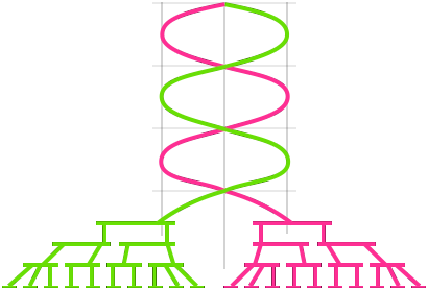
\includegraphics[width=4.5cm]{img/untangled}
\end{wrapfigure}

In a traditional top-down proof search based on a system of inference rules, the prover must reach the system's \emph{axioms} --- rules with no logical premises ---
in order to seal off a proof branch.
Only following successful closure of all proof branches can the prover declare victory.
Two major factors contribute to search-space explosion:
the proof \emph{width}, caused by having multiple rules be applicable at any given point in the proof;
and proof \emph{depth}, caused by the long chain of rules that have to be applied, consecutively, in order to reach the axioms from the proof goal.

%\todo{The key ingredient here is that when searching top-down, you need to reach axioms in the leaves; when combining bottom-up, you can stop earlier when you have reached a lemma that was discovered previously.
%More importantly, the lemma can be discovered by a variety of proof techniques, which can be SMT- or ATP-driven.}
Our modularization approach for more effective theorem proving is based on the introduction and use of \emph{ancillary lemmas}, encapsulating some details of the proof and reducing the search depth by providing a wider range of known facts that can be used as leaves.
Such lemmas are typical in mathematical pen-and-paper proofs, and they are layered on top of one another to be able to convey a complex development.
To amplify the significance of lemmas we propose a novel approach to problem decomposition, called \textbf{untangle-and-conquer}.
As the name suggests, it consists of two phases, the first of which is aimed at splitting a proof goal such that each sub-proof can be comfortably completed using an existing database of lemmas.
We identify the following gap: logical propositions occurring as proof goals contain a mixture of logical symbols from different theories.
For example, they may contain operations on arrays as well as linear arithmetic over the indices and pointer operations on the elements.
In contrast, lemmas are naturally smaller and involve only a handful of symbols.
This applies to both human-constructed lemmas, because the cognitive load required to deal with intricate interactions between too many different concepts is high;
and to automatically generated lemmas (which we discuss shortly), since large vocabularies incur high resource costs to search through.
It is therefore desirable to engineer the proof in such a way, that each part contains a subset of the symbols occurring in the goal.


Oftentimes, choosing the right lemmas to use as stepping stones is the key insight a mathematician has to come up with.
It would definitely be presumptious to expect an automated reasoning program to replicate this much insight; but there are two key factors working to our advantage when dealing with software-oriented proofs:
(i) Even if some lemmas require ingenuity in their formulation, there is an even larger number of simpler, more ``mundane'' lemmas, and finding those automatically removes tedium from the human user;
(ii) Lemmas used in different proofs are often similar, 
so building a database of discovered lemmas can help the prover in future endeavors;
(iii) By the same argument, using a corpus of previously completed proofs (either human- or machine-generated) can guide the search for lemmas and make use of past results.

We are especially interested in \emph{theory exploration} (or \emph{theory forming}):
Given a library of proven properties, an automated reasoning system can eagerly search for consequences, thereby growing the body of ``knowledge'' at the prover's disposal.
Deductive proof search in ATPs such as Vampire and Cyclist tends to be oriented ``top-down'', that is,
starting from a proof goal, simplifying it further and further until axioms are reached.
The is analoguous to building the proof tree from the root down to the leaves. (Although, graphically, proof trees are commonly depicted with the root at the bottom --- this is nevertheless a top-down approach.)
The availability of synthesis technology \cite{quickspec,thesy} means that we can generate a vast number of lemmas to guide our untangle-based decomposition.
The major risk here is that too many lemmas may incur a high overhead and, moreover, produce too many different ways to decompose a given proof.
We propose to mitigate this by developing a ranking method for discovered lemmas based on their usefulness,
so that our automated reasoning tool can \textbf{learn from experience} and get better over time, using classic statistical inference.
\end{paragraph}

\begin{paragraph}{Objective 4: {\it Extrapolating to Software}}~
The overarching goal of this research is to pave the way for the next generation of theorem proving technology.
The emphasis remains on making tools that allow reasoning about properties of computer programs.
What this means is that an automated prover is required to cope with a high volume of low-level details that interact in unexpected ways.
We would like to take advantage of \textbf{inherent abstraction layers} that already exist in software,
since abstraction is what makes it possible
for human programmers to cope with its ever-growing complexity.
One form of abstraction can be used via the ancillary lemmas described above.
An orthogonal axis is the application of \textbf{semi-automatic refinement} to provide encapsulation for some of the implementation details.
For example, an ordered data structure may be abstracted as a set and a (total or partial) order relation; a multi-threaded process may be abstracted as a sequential one that is behaviorally equivalent.
Choosing the abstraction to use in a refinement proof would, more often than not, require some human intuition, which is why some amount of user interaction will be needed.
Our hope is that with the right abstraction in place,  the automated prover will be able to carry out all or most of the refinement proofs,
showing that the abstraction soundly models the underlying implementation and also inferring system invariants from it --- making this process extremely rewarding.
\end{paragraph}


\begin{comment}
% I am not sure what to do with this
Another obstacle, which hinders both approaches, is the use of quantification
in assumptions and theorems.
One generally wishes to take advantage of the inherent modularity in proving
most kinds of properties, be those mathematical theorems in algebra or combinatorics,
and definitely when it comes to correctness properties of computer programs.
Software is modular by nature, 
It is very much desirable to adopt the same contributing factor to reasoning about
these programs.
This means that instead of constructing one monolithic proof of the ``ultimate
theorem'', one identifies and proves \emph{lemmas} that abstract and generalize
domain knowledge and understanding of the underlying program --- layering them
up until the final goal is met.
This is definitely how it is done in academic papers, and, more recently, in
large software verification projects.
Going back to the challenge at hand, these auxiliary lemmas typically include
quantified formulas, which are logic's way of expressing generalized conjectures.
Applying these lemmas, \eg in the context of carrying out the next step of the proof,
ultimately requires to instantiate universal quantifiers with logical terms.
Since the space of available terms is large (or even infinite), this becomes
a task that is daunting to automate and requires the employment of heuristics
to select the right instances.
We will move to consolidate instantiation strategies into ones that more closely
matches the search for proof --- thus being goal-directed rather then origin-directed.
A primary aim is to make these strategies less heuristic and more predictable.
\end{comment}

\section{Research Plan \todo{B2}}

\subsection{Inductive-Deductive Reasoning Hybrid}

Deductive reasoning is the practice of applying general rules or statements to
individual, concrete cases; conversely, inductive reasoning is one of inferring,
from a set of observations, a unifying generalization.
Deductive reasoning can be thought of as a ``top-down'' application of logical
thinking, whereas inductive reasoning works ``bottom-up''.
While inferring a special case from a general case is always logically sound,
generalizing from examples can only guarantee soundness up to the set of
instances observed.
Still, even in the course of proving theorems, where soundness is of utmost
importance, humans habitually make use of inductive reasoning to guide their
deduction:
just a handful of examples can give rise to a useful generalization, a lemma,
which can then be proven deductively.

While there is no perfect analogue in the prover/solver setting as portrayed
in \autoref{intro}, it is quite obvious that theorem provers employ deductive
reasoning almost exclusively.
It would be inaccurate to say that SMT solvers employ inductive reasoning in
the same sense; a lot of their mechanics is still based on deduction.
However, they are very much oriented toward constructing a model of the given formulas.
State-of-the-art SMT solvers make use of (partial) models generated in the
course of the search to guide deductive reasoning as this search progresses.
One notable example for this is Model-Based Quantifier Instantiation (MBQI),
a technique implemented in Z3.
In Sketch, a software synthesis tool, the system observes a set of inputs (and
outputs), proposes a generalization (a program), and then attempts to verify it
using a deductive method (in their case, reduction to SAT).\todo{what no, need to explain the use of counterexamples}
A growing number of examples is needed for the generalization to yield a correct
program, so this process repeats in a loop.

The idea of accumulating models of formulas or sub-formulas in the course of
a dialog between a deductive component and an inductive one can be lifted to
any type of reasoning.
When constructing proofs, existing models can be used to quickly vet possible
branching choices and discard ``obviously wrong'' ones: it is clearly futile
to try to prove a formula that is not valid, and any instance that does not
satisfy it can serve as a witness for that.
This is very much the process that a human mathematician may undergo when
considering which conjecture to prove next.
Clearly, having a representative set of models is essential for it, since
most intermediate statements have the form ``if $A_1$ and $A_2$ and $A_3$, then
$B$'', and models not satisfying one of the premises $A_i$ contribute no
relevant information.
It is thus desirable to identify ``pivot'' atomic formulas and keep around
models for various subsets of them.


\subsection{Unification Modulo Theories}

Theorem provers offer the flexibility that comes with customizing the logic used and its inference rules.
This makes it possible to encode high-level strategies for problem decomposition, and incorporate domain knowledge for different classes of problems.
What ATPs are not good at---in some cases, in fact, pretty bad---is
handling many different cases requiring sub-proofs,
as is the situation when, \emph{e.g.}, observing a computer program with several conditional statements.
SMT solvers, on the other hand, evolved around the SAT problem and are therefore better equipped to cope with issues of Boolean structure.

\begin{figure}
\centering
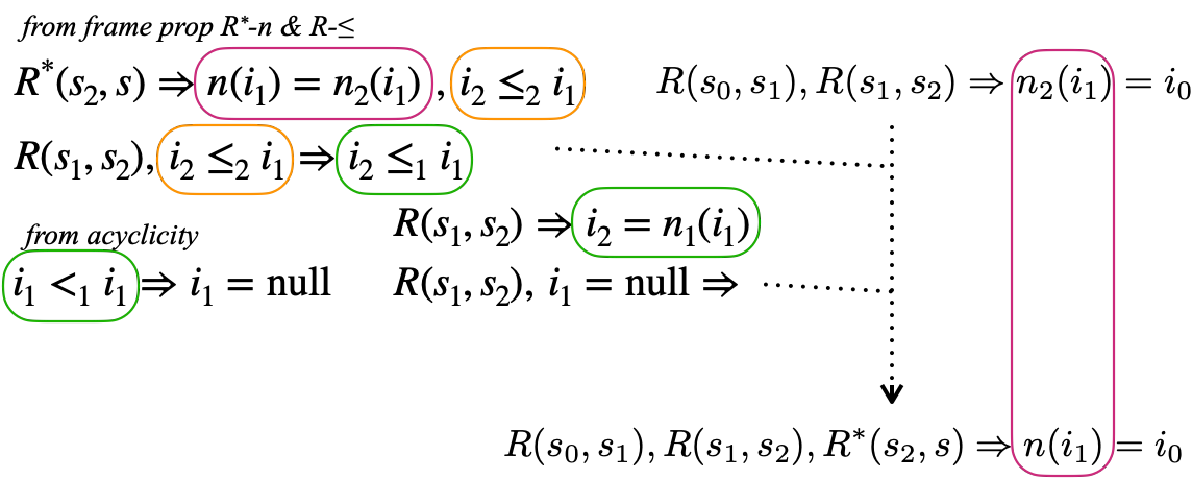
\includegraphics[width=0.75\textwidth]{img/unification-modulo-theories.pdf}
\caption{}
\label{unification:example}
\end{figure}

To facilitate effective proof search in a tool that combines the strengths of both ATP and SMT,
we propose a technique that involves dedicated theory solvers directly in the process, rather than having a narrow interface through which they communicate their results.
A core mechanism in deductive inference is that of \emph{unification}, where formulas from the goal are checked against known sequents that were previously derived to see if these sequents can fill in some pending premises.
Since both the goal and the pre-existing sequents may contain free variables, this procedure is not merely checking equality, but also provides substitution and renaming of variables when needed.
The proposed development is to enhance the unifier with knownledge about background theories, such as the theory of equality, partial orders, group theory, and transitive closure (the latter described below in \todo{}).
This would allow the unifier to not only detect syntactic matches, but also consider situations where an existing formula entails a given premise according to the theory,
and also combine several facts to satisfy one such premise.

An example illustrating how this may affect proof search is given in~\autoref{unification:example}.
The current goal is
$R(s_0,s_1), R(s_1,s_2),R^*(s_2,s) \Rightarrow
n(i_1) = i_0$,
and the pre-existing fact is
$R(s_0,s_1), R(s_1,s_2) \Rightarrow n_2(i_1)=i_0$.
A-priori, the sequents cannot be unified, because the goal has $n(i_1)$ on its right hand side, whereas the fact has $n_2(n_1)$.
Instead of giving up on using the given fact at this point, the prover can then deduce that $n(i_1)=n_2(i_1)$, thus utilizing the theory of equality.
Establishing $n(i_1)=n_2(i_1)$ itself requires some extra reasoning, since the given sequent in the prover's collection of known facts is, in this example,
$R^*(s_2,s)\Rightarrow n(i_1)=n_2(i_1), i_2\leq_2 i_1$.
The precondition $R^*(s_2,s)$ is already present, luckily, on the left-hand side of the current goal;
however, the literal $i_2\leq_2 i_1$ must be eliminated before the equality can be utilized.
This is a sub-task in which SMT solvers shine:
the right-hand side of the fact is essentially a disjunction, and the solver can perform a case split and eventually discover that $i_2\leq_2 i_1$ contradicts other known properties, listed below in the figure.
During this process of elimination, an acute role is played by the literals $i_2\leq_1 i_1$, $i_1<i_1$, $i_2=n_1(i_1)$ and the underlying theory of transitive closure.

\subsection{Feasible Induction Through Transitive Closure}

In the spirit of the mechanics of SMT solvers, where different \emph{theory solvers}
can be combined using methods such as DPLL(T), CDCL(T), and Nelson-Oppen, we
propose an important module would be a solver specifically capable of reasoning
about transitive closure properties.
Particularly, this solver will be able to construct models of quantifier-free
FO(TC) formulas.
FO(TC) is an extension of first-order logic with the addition of atomic formulas of the form $\big(\mathrm{TC}_{x,y}\varphi\big)(s,t)$,
whose semantics is the existence of a path $s=u_0,u_1,\ldots,u_n=t$, $n\geq 1$, with $\varphi[u_i/x,u_{i+1}/y]$
holding between all pairs of successive elements.
$x$ and $y$ are supposed free variables in $\varphi$, so $\varphi$ is commonly thought of as representing a binary relation, and $\big(\mathrm{TC}_{x,y}\varphi\big)$---the transitive closure of this relation.
A commonly used variant is $\big(\mathrm{RTC}_{x,y}\varphi\big)$, with the only difference being that $n\geq 0$ (instead of $1$),
which in turn induces the \emph{reflexive} transitive closure.
Another extension allows relations of arbitrary even arities
$\big(TC_{x_1,\ldots,x_k,y_1,\ldots,y_k}\varphi\big)$;
this transitive closure can be thought of as a path between $k$-tuples, where $x_1,\ldots,x_k$ and $y_1,\ldots,y_k$ represent coordinates of adjacent tuples.
In the sequel, we use the phrase ``transitive closure'' as an umbrella term for these closely related variants.

The proposal is to ingrain the notion of transitive closure in the language and proof search procedures of automated theorem provers.
The first expected benefit of this is that transitive closure enables clean, compact representation of data-related properties,
making the logic easier to use and the resulting formalisms clearer.
For example, the classical construction of the natural numbers from first principles involves a zero element and a successor operator.
Based on this definition, operations and relations over natural values, such as the order relation $\leq$, can be defined via induction/recursion.
\[
\begin{array}{l@{\hspace{4em}}l}
\begin{array}[t]{l}
\rInductive~\tnat~\eqdef \\
\quad |~0 : \tnat \\
\quad |~S : \tnat \to\tnat
\end{array}
&
\begin{array}[t]{l}
\rInductive~\fle : \tnat \to \tnat \to \tProp ~\eqdef \\
\quad |~\fctorlen : \forall n:\tnat,~ \fle\,n\,n\\
\quad |~\fctorleS : \forall (n\,m:\tnat),~ \fle\,n\,m\to\fle\,n\,(S\,m)
\end{array}
\end{array}
\]

The definition of $\fle$ is amongst the most basic ones in Type Theory; yet it commonly baffles newcomers and takes some time convincing that it indeed defines the familiar notion of $\leq$.
Using transitive closure, however, offers a more compelling formulation:
\[
\fle\,x\,y ~\eqdef~ \big(\RTC{x,y}\,S\,x=y\big)(x,y)
\]

The above formula reads: $x\leq y$ iff $y$ can be obtained from $x$ by zero or more application of $S$, the successor function.
This naturally aligns with our fundamental perception of ordering of natural numbers.
In this sense, the transitive closure construct captures a recurring pattern in recursive definitions, one that seasoned TT users can identify at a glance, but which nevertheless adds some amount of unnecessary ``noise'' to the mix.
This noise becomes more significant as definitions grow in complexity, and eventually encumbers proof search and development.
In particular, chained application of a previously defined function or relation is so commonly useful, that it makes sense to define a designated notation for it:
\[
\fle\,x\,y ~\eqdef~ x[S^*]y \hspace{4em}
\textit{where:}~
\begin{array}[t]{l}
  {} [f] : D\to D\to\tProp ~\eqdef~ \lambda x\,y, f\,x=y \\
  {} [R^*] ~\eqdef~ \big(\RTC{x,y}\,R\,x\,y\big) \\
  {} [f^*] ~\eqdef~ \big[[f]^*\big]  \qquad\textrm{\small(\textit{and analogously for} ${[]}^+$)}
\end{array}
\]

The use of square brackets in notations occurring in this document helps to avoid ambiguous expressions, and also provides an opportunity for using binary relations as infix operators;
\eg, we write $x[S^*]y$ as a more elegant alternative to $[S^*]\,x\,y$.

\begin{figure}
\begin{center}
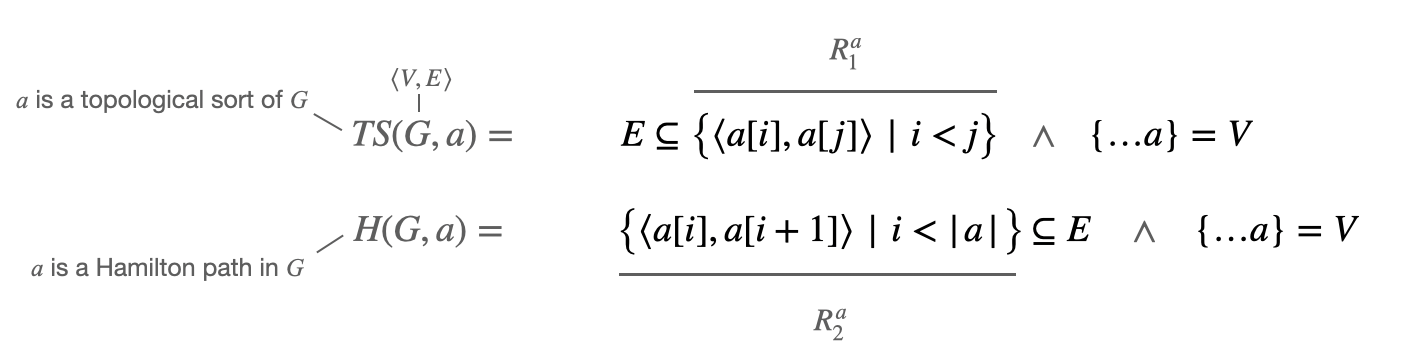
\includegraphics[width=.8\textwidth]{img/topological-and-hamilton.png}
\end{center}
\todo{typeset with $\fTS\,G\,a$ and $\fH\,G\,a$}
\caption{Formal definitions of topological sort and Hamilton paths
  for use in \autoref{plan:hamilton}.}
\label{plan:hamilton-defs}
\end{figure}

We argue that the compact TC formulation allows for shorter proofs---which in turn lead, potentially, to easier proof derivation processes in both interactive and fully-automated settings.
We use the following example to illustrate this point; it is a problem taken from an undergraduate class on algorithms.

\begin{example}~\label{plan:hamilton}
\begin{tabular}[t]{lp{10cm}}
\textit{Given:} & A directed acyclic graph $G=\langle V,E\rangle$.
\\
\textit{Task:}  & Determine whether the graph contains a \emph{Hamilton path}; \ie, a (directed) path that visits every $u\in V$ exactly once.
\end{tabular}

\medskip
This exercise is given following a lecture on DFS, BFS, and topological sort.
This gives rise to a short solution:
(1)~topologically sort the vertices of $G$;
(2)~check whether the resulting array constitutes a path,
 that is, every two consecutive elements are connected by a path.
 
While the algorithm looks simple, it is not at all obvious that it is correct w.r.t. the requirements.
Clearly, if it returns $\ftrue$, then it has correctly discovered a Hamilton path (even without considering any properties of topological sort).
But when the outcome is $\ffalse$, some acute reasoning is required to show that there does not exist a \emph{different} ordering of $V$ that will indeed corresponds to a Hamilton path.
To establish correctness, the student needs to formalize the definition of topological sort and that of a Hamilton path
(\autoref{plan:hamilton-defs}).
Then the following proof goal must be accomplished:
\begin{equation}\label{plan:hamilton-goal}
\fH\,G\,a,~\fTS\,G\,a' ~\vdash~ a = a'
\end{equation}

That is, in a DAG containing a Hamilton path, there is exactly one possible topological sort, and that sort is identical to the order imposed by the Hamilton path.
(Notice that a DAG may contain at most one Hamilton path; this property is obtained as a simple corrollary of (\ref{plan:hamilton-goal}).)

An insight into the proof can be offered by considering the two binary relations $R_1^a$, $R_2^a$ occurring in the definitions of $\fTS$ and $\fH$.
A keen observer can notice that: $R_1^a = [R_2^a]^+$.
The implication would be that the topological sort ($R_1^a$) is uniquely determined by the Hamilton path ($R_2^a$) if the latter exists.
From there, proving (\ref{plan:hamilton-goal}) is by no means routine, but it does follow from rather standard algebraic conjectures:
\begin{enumerate}
  \item $R_1^a$ is a \emph{total order} on $V=\{\ldots a\}$.
  \item A total order is \emph{maximal w.r.t. set inclusion}
    over all (partial) orders on the same set.
  \item The mapping $a \mapsto R_1^a$ is \emph{injective}.
\end{enumerate}

Notably, the monotonicity of the transitive closure operator $^+$ (as of any closure operator) is utilized here to establish the relationship $R_1^a \subseteq R_1^{a'}$.
In this small instance, it is completely reasonable to expect that an automated prover can infer the three auxiliary properties listed above, as well as construct their proofs, without the user's intervention.
In more complex scenarios, the aspiration is toward the prover and the user working hand-in-hand, with the prover suggesting some conjectures that can progress the proof, and the user selecting the ones that make the most sense while also adding propositions that were not automatically discovered.
The use of algebraic concepts here is deliberate: the phrases ``total order'', ``set inclusion'', ``injective mapping'' all encode knowledge previously gained from human experience in defining and solving mathematical problems.
\end{example}

\todo{describe the objective and how the transitive closure solver fits in the general scheme}

\begin{figure}
\begin{center}
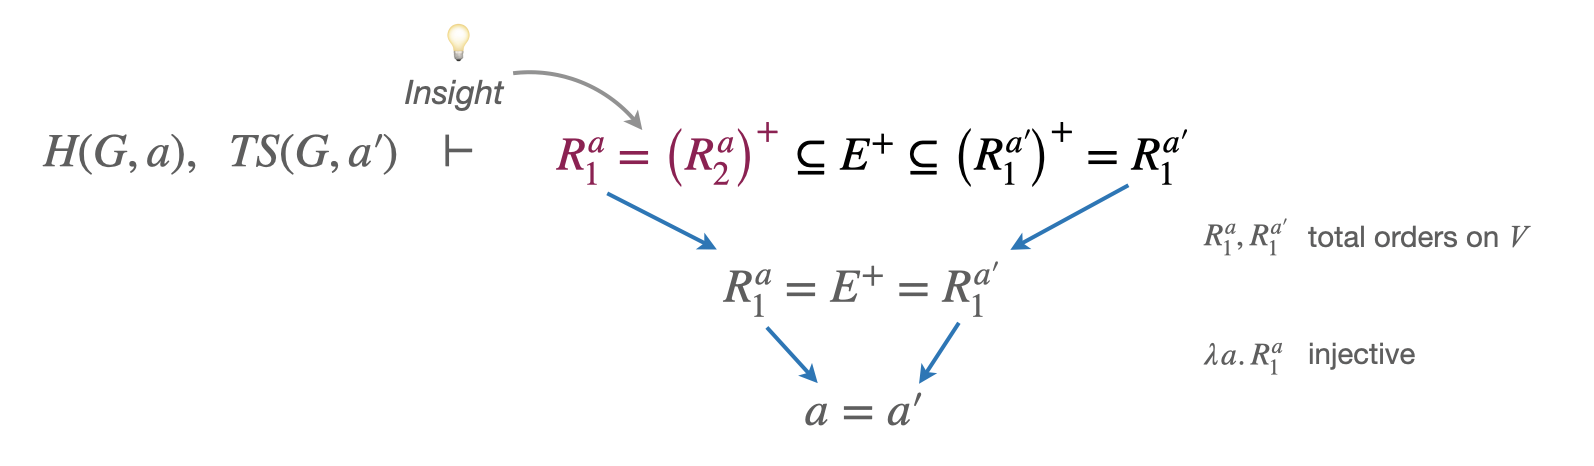
\includegraphics[width=.8\textwidth]{img/topological-and-hamilton-proof-sketch.png}
\end{center}
\todo{typeset with $\fTS\,G\,a$ and $\fH\,G\,a$}
\caption{A sketch of the proof described in \autoref{plan:hamilton}.}
\label{plan:hamilton-proof}
\end{figure}

\subsubsection{Using Implicit Induction}

Most theorem provers, as well as some SMT solvers and systems using them,
prove inductive properties by the introduction of an \emph{induction scheme} ---
a specialized inference rule, whose premises comprise the induction base case
and step.
For example, given $P(0)$ and $\forall k.~ P(k)\rightarrow P(k+1)$,
one can infer $P(n)$ for any natural $n$.
In this way, the induction step effectively ``hides'' several application of
the induction hypothesis $P(k)$ inside a single inference step.
This is much different from the way humans approach the problem: they may set
out simplifying $P(k)$, realizing at some point that it may follow from $P(k-1)$,
justifying such reasoning based on the natural numbers being a wellfounded set.

\todo{this is the completely wrong setup. it has been shown to be effective already, it is no longer a conjecture.}
{\color{gray}We conjecture that this \emph{implicit} induction approach is suitable for
automatic proof discovery as well.
The formal implementation in this context is that of \emph{cyclic proof systems};
the cyclic framework admits proofs where some premises are satisfied by
conjectures occurring \emph{later} in the goal.
Of course, for such proofs to be sound some side conditions are imposed to assure
that a wellfounded order can be established.
}

\subsubsection{Overcome the Frame Problem with Frame Properties}

A prevalent difficulty of reasoning in logic is the \emph{frame problem}:
a constant need to specify not only effects we are interested to reason about,
but the entire environment surrounding it, which was not directly affected.
In the context of reasoning about computer systems, a program may effect a change
by storing or removing some data, causing a change in the system's state.
In order to prove properties of the system, and in particular, of such
accumulated changes, logic dictates that we formulate precisely what has
\emph{not} change in the system's state, including memory locations, database
tables, network communication packets \etc, that the program did not touch.
This is a huge hinderance to effective reasoning since properties that were
assumed or already proven with regard to the input state, have to be
re-stated and proven respective to the new state.
Such proofs are mundane and daunting, but there are many such properties
popping up in the course of a proof and they may very well require more work to
discharge than the ``insightful'' part.

\begin{figure} 
\begin{lstlisting}[basicstyle=\linespread{1.36}\ttfamily\fontsize{10pt}{8pt}\selectfont]
reverse(h) :=
  i := h; j := null;
  while (i != null) {
    t := i.next;
    i.next := j; j := i;
    i := t;
  }
\end{lstlisting}
\end{figure}

A classical example for the severity of the problem is analysis of the program
\textsf{reverse}, which reverses the order of nodes in a singly-linked list.
The program flips one edge at a time, and the effect of each iteration is
very local; however, to prove even a most basic property, that the program does
not introduce cycles in the list, the programmer has to include properties of
the prefix and suffix of the list, which have not changed --- the ``frame''.
The bookkeeping difficulty was so intense, that it led John C. Reynolds to the
conclusion that reasoning about pointer paths using transitive closure (heap
reachability) is not practical, and to found a new logic for dealing with
programs with dynamic heaps.
This logic is known as Separation Logic and is still the state-of-the-art in
reasoning about heaps.

%\begin{figure}
%\includegraphics[width=5cm]{standalone}
%\embedlatex[width=5cm]{standalone}
%\end{figure}

We claim that transitive closure \emph{can} be made effective by harnessing
\emph{frame properties} arising from the theory of transitive closure.
Frame properties are theorems and lemmas that assert the preservation of
certain properties, across consecutive program states, subject to the more
fine-grained properties preserved by the transition between them.
Frame properties can be generic or specific; \emph{generic} frame properties are
schemas that can apply to any $\varphi$ formula occurring within a transitive
closure $\big(\mathrm{TC}_{x,y}\varphi\big)$.
\emph{Specific} frame properties pertain to concrete programs and their respective
state transition semantics expressed as formulas.
An example of a generic property is: if there is a $\varphi$-path between some
two individuals $u, v$, and if for any $x,y$ $\varphi$-reachable from $u$, it
holds that $\varphi(x,y) \leftrightarrow \psi(x,y)$, then there is also a
$\psi$-path between $u, v$.
A derived, specific frame property could be the following: assume $n$ is a
function symbol representing the pointer links of a linked list, and assume
$n'$ is another function symbol representing the links of the same list after
a \emph{single iteration} of the program \textsf{reverse}.
Then all nodes reachable from the \emph{successor} of the loop iterator in the
former list, are still reachable from it in the second list.
This follows from the fact that the location of the modified pointer is not
reachable from any of the nodes in question, so the link paths in that area of
the list (the suffix) could not be affected.

\todo{example for frame property(-ies) in TC}

\begin{figure}
\centering
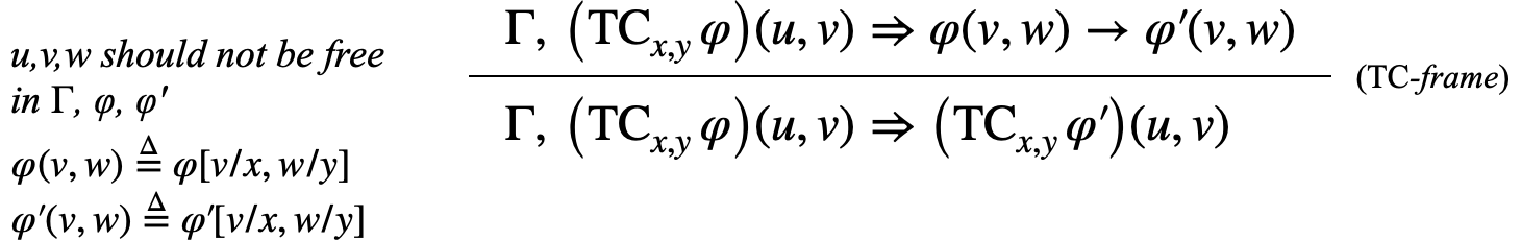
\includegraphics[width=10cm]{img/tc-frame-gen.pdf}
\caption{Generic frame property for (reflexive) TC}
\end{figure}

By developing proof-support tools that ``guess'' specific frame properties
% xref lemma speculation
and prove them automatically based on more primitive facts and by applying
generic frame properties, we expect to greatly improve the efficacy of theorem
provers and also of interactive proof assistants in handling conjectures
involving transitive closure.
While frame properties do not, formally, play any special role compared to
other formulas occurring throughout the proof, they follow a unique kind of
``thought pattern'' that serves a mental purpose in abstracting away nitpicky
details.
This would allow us to focus human and machine attention alike on the more
nitty-gritty parts of the proof.

\subsubsection{Next-level Transitive Closure}

The use of transitive closure logic is not restricted to reasoning about heap
graphs, which mostly involved low-level kind of reasoning.
Many aspects of computing rely on iteration, \eg when expressing properties of
aggregate data --- a sum of a column in a database, for instance.
Indeed, there is a large and interesting space of programs that can be realized
with the combination of the functional operations \textsf{map}, \textsf{filter},
and \textsf{reduce}. % cite SPARK
Sets and sequences can be stored in many ways in memory and in non-volatile
storage, yet the iteration aspect remains the same and can be characterized by
a ``next-in-iteration'' function that matches for each element, the following
element in the iteration order.
The loopy construct, \eg sum, can then be axiomatized using the transitive
closure $\big(TC_{\langle a,u\rangle,\langle b,v\rangle}v=n(u) \land b=a+\mathrm{val}(u)\big)$
With the help of TC support in the theorem prover, and in the presence of a
library of theorems defining known properties of TC, reasoning about such
aggregates can be streamlined to be simpler than by using the corresponding
inductive definition of sum.
For example, distributivity of sum over sequence concatenation follows (almost)
for free from the transitivity of TC.



\subsection{Modular Reasoning with Lemmas}

Mathematical proofs are seldom monolithic.
Usually, there are some intermediate conjectures --- \emph{lemmas} --- that
are proved one by one, gradually building toward the culmination of the main
theorem.
It is not done out of altruism towards potential readers of the paper, though it can
certainly make a proof easier to understand.
Mainly, it helps the author overcome the complexity of the proof development
task: in a formal setting, even a seemingly benign logical step can have many
inference steps; and the steps are not always sequential, for example when
a case split is required in order to consider several scenarios.

This kind of modularization has been carried over by computer scientists to the
realm of interactive proof assistants.
In Type Theory, the use of lemmas is wired in as they are reduced to function
calls following the Curry-Howard Correspondence.
Modular proofs are even more of the essence in automated proof search, due to
the inherent computational complexity of the tool and poor scalability of
existing search techniques.
Breaking a proof task into lemmas also carries the promise of combining different
approaches to finding the proofs, by applying a portfolio approach in the spirit
of Why3 \cite{}.

\subsubsection{...}

\subsubsection{Near-match Lemma Speculation}

The following is a common scenario for anyone who has worked on formal proof development:
you have a conjecture to prove, and there is
a theorem whose conclusion seems to fit the conjecture, but does not \emph{quite} match.
As a very simple example, suppose the conjecture is
$\exists k.~ n = 2\cdot k$, and the preexisting theorem states:
\begin{equation}\label{manna-divmod}
  \forall i, j.~ i = \fdiv(i, j) \cdot j + \frem(i, j)
\end{equation}

(Inspired by Manna and Waldinger, 1980.)
Strict syntactic unification would fail to apply (\ref{manna-divmod}) to the proof goal $n = 2\cdot \evar{k}$, since (\ref{manna-divmod}) has a $+$ operator on the right-hand side of the equality.
(Here and in the sequel, we use $\evar{k}$ to designate a pattern variable that can be unified with anything.)
However, an intelligent mathematician knows that according to the basic laws of arithmetic, $\forall x.~x + 0 = x$.
It is possible to ``unblock'' the unification process if we equate $\frem(\cdot,\cdot) = 0$.
Similarly, unifying $\fdiv(n,\evar{j})\cdot \evar{j}$ with $2\cdot \evar{k}$ would fail, since $2$ cannot be unified with $\fdiv(n,\evar{j})$.
Again, by the law of commutativity, 
$\fdiv(n,\evar{j})\cdot j = \evar{j} \cdot\fdiv(n,\evar{j})$,
so we should be able to unify $\evar{j}$ with $2$ and $\fdiv(n, 2)$ with $\evar{k}$.

This process of \emph{unification modulo equalities}, or \emph{E-unification}, has been explored in the past but never exploited for automation\citeneeded{}.

{\color{gray}
transitive closure (see above) of a unary function $n$.
Transitivity dictates that this follows from $n^*(x,v), n^*(v,z)$ for some $v$,
and there is an assumption, or a previously proven conjecture, $n^*(x,y)$;
however, no assumption $n^*(y,z)$ is available.
Instead, what you have is $m^*(y,z)$ for a second function $m$.
This can be overcome by proving that $m^*(y,z) \Rightarrow n^*(y,z)$, as a
separate lemma.
To prove such a lemma, one may try to prove that $n=m$, or that $n^*=m^*$,
or that $\forall u, n^*(y,u)\leftrightarrow m^*(y,u)$, or any other generalization
of the missing implication.}

To mechanize the process, a prover is required to select a suitable version.
Some alternatives can be vetted out using the model-based approach described
earlier.
Proving the auxiliary lemma can also be postponed to a later stage, after the
prover has concluded the current proof branch and admitted it --- since a failed
proof branch will be discarded anyway, and all the lemmas used in it become
moot.
Hence the term ``speculation'', also used in works on proofs by rippling \cite{}.
In the original presentation, speculated lemmas are equalities between terms,
but they can be made far more general and integrate
into any kind of clause-based inference system such as natural deduction or
sequent calculus used by modern provers.


\subsubsection{Semi-eager Theory Propagation}

The T of SMT stands for \emph{Theory}.
A theory in this context comprises of a specific vocabulary, inducing a limited
subset of logical formulas, and a designated interpretation, thus also limiting
the logical \emph{structures} that can be considered for them.
One popular example, built into many SMT solvers, is the theory of integer linear
arithmetic (LIA): it provides the operators ``$+$'', ``$-$'', ``$\cdot$'' as
well as order relations ``$=$'', ``$\leq$''.
It imposes a syntactic restriction that two variables may not be multiplied;
a variable may only be multiplied by a constant numeric literal.
While a formula such as $5 < 3$ is \emph{logically} satisfiable, it is
unsatisfiable in the theory of LIA, since it requires all numeric literals to
be interpreted as the integers they represent and that ``$<$'' be interpreted
as the order of integers.

Communication between the SAT component and the theory component of the model
is handled by the theory solver producing \emph{learned clauses} that are valid
modulo the theory and a logically unsatisfiable when conjoined with the existing
goal.
For $5 < 3$, this may be as simple as $\lnot(5 < 3)$; but the clauses get more
involved as problem sizes and number of variables grow.
The generation of clauses by the theory solver is called
\emph{theory propagation}, and can be done in two ways: (i) \emph{eagerly}, by
observing the formula given to the solver and generating all the theory-valid
statements containing the terms it contains; and (ii) \emph{lazily}, waiting for
SAT to produce a Boolean assignment and then contradicting it with
appropriate clauses when it is inconsistent with the theory.

The eager approach has an inherent flaw: the number of such theory-valid
statements can grow very large very quickly.
It can be infinite, in the case of some theories, as most theories are
represented, conceptually speaking, by quantified formulas, and there is no
bound on the number of instantiations that may be needed to refute a single
statement.
Some theories, in particular those of integers, are not even definable by any
finite set of first-order formulas, quantified or otherwise.
Such difficulties cause eager propagation techniques to be all but abandoned.

The lazy approach, despite its popularity, can have severe run-time
implications.
It means that a number of SAT assignments have to be observed, and a
potentially computation intensive procedure consulted, to refute their
satisfiability in the logic.
Designers of SMT try to be clever in the way propagation clauses are generated,
since generating more general clauses will drive the SAT away from more
inconsistent assignments at an earlier stage, saving calls to theory solver.
This tactic is limited, however, since the theory solver only gets a glimpse
of a narrow case each time it is involved, and cannot make global decisions
based on the structure of the entire input problem.

We propose a middle ground, and that middle ground involves a more holistic view of the proofs.
In a combined setting where SAT, theories, and formal proof objects work
together, intermediate proofs being explored provide ample subformulas to
fertilize propagation.
We will define an \emph{integration metric} for propagation clauses, that
quantitively expresses how tightly coupled a potential clause is with the
existing set of assumptions and goals present in the proof.
This can be thought of as a miniature ``page rank'' for logical formulas:
``hot'' atomic formulas, that is, ones that occur often in the proof, encourage
clauses that contain them, and these clauses, if accepted, will light up
more atomic formulas, with rank diminishing as they drift further from the
core.
Then, we will construct effective algorithms for finding such clauses that
optimize this metric.
We will tune the metric and the algorithms to achieve the fastest convergence
and compare to existing heuristics.

This semi-eager propagation of clauses from theories hold true potential for
a breakthrough with respect to handling theories and quantified conjectures
in unison, as challenged by Voronkov \citeneeded{}.


\subsubsection{Lemma Patching}

Again, this is inspired by the way mathematicians work, first proving a
simplified version of a desired property as a lemma, then inspecting the proof
to figure out ``what would go wrong'' in the more general case --- using that to guide insight toward
proving a stronger lemma.
Intermediate proofs are thus raw material for more proofs: this lends a
``white-box'' view of lemmas, complementing the more basic use of lemmas in
their closed form, encapsulating their proofs (which can be seen as
``black-box'').
In a dual manner, occasionally a lemma is too strong: \eg, if its conclusion is
a conjunction, but one is only interested in one of the conjuncts.
It is possible that a subset of the premises is sufficient to prove that one
conjunct.
Another example is when a conclusion is of the form $a < b$, but a relaxed set
of premises is enough to obtain $a \leq b$.

Moreover, during proof exploration itself (either by human or by machine), some
incorrect, dead-end proofs are inevitably encountered.
These are characterized, indeed identified, by assumptions that cannot be made
soundly (\eg a proof branch that includes formulas that are not logically valid).
Normally, a theorem prover simply discards these failed attempts and tries
other directions.
However, these too can be leveraged as raw material; repairing them amounts to
eliminating the spurious, invalid assumptions.

\begin{figure}
\centering
\raisebox{-.33\height}{
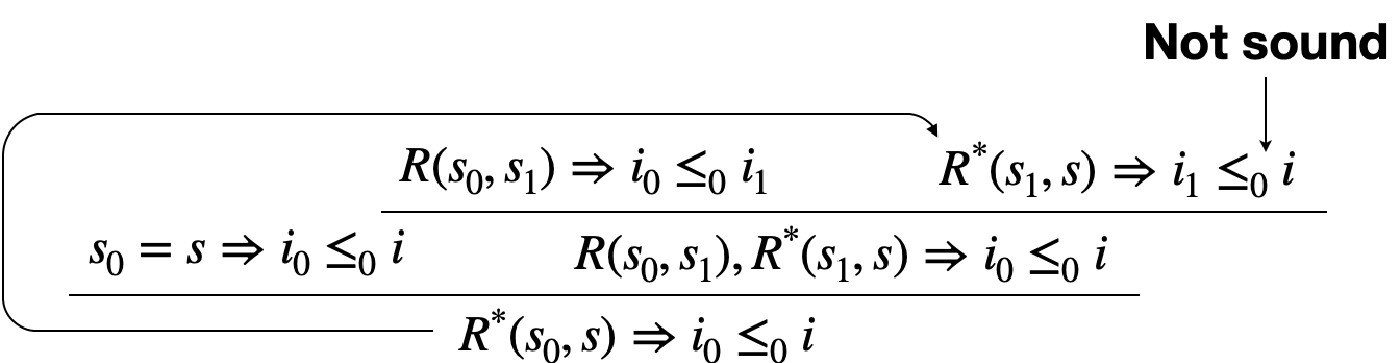
\includegraphics[width=7cm]{img/lemma-patching.pdf}}
$\longrightarrow$~~
\raisebox{-.33\height}{
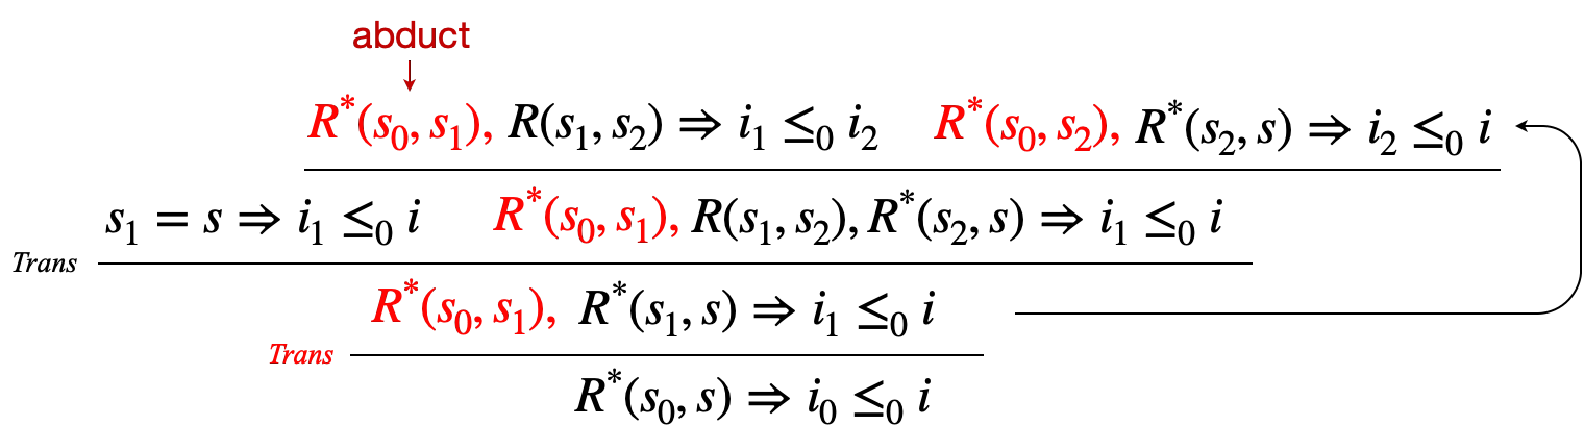
\includegraphics[width=7.5cm]{img/lemma-patching-abduct.pdf}
}
\caption{Example for lemma patching}
\label{lemma-patching-example}
\end{figure}

\todo{refer to \autoref{lemma-patching-example}}


\subsection{Extraploating to Software}

As much as mechanical theorem proving is useful for formalizing mathematics, it has much wider and more exciting uses when it comes to reasoning about computer programs and their semantics.
To date, the most popular text on interactive theorem proving in Coq is the Software Foundations series~\citeneeded{}, a collaborative community
effort to formalize programming language concepts
and verification problems.
The example proofs and exercises in the textbook make some use of proof automation facilities existing in Coq.
These are, however, far from what can be offerred by dedicated automated provers and solvers.
This research aspires to bring such automated tools to a new level, in which they will be able to cope with these fundamental tasks naturally and directly.
Most importantly, that they will be capable of handling such formal definitions as occur in~\citeneeded{(SF again)} naturally, without requiring the user to translate their claims into a restricted logical fragment.

\subsubsection{Homotopy for Programs}

Homotopy Type Theory~\citeneeded{} is an emerging field of study offering a fresh view on Martin-L\"of  Type Thoery, in which type judgements are given
first-class-citizen status.
Types can be declared isomorphic, allowing terms of one type to be interpreted as the other type.
In the field of mathematics, homotopy is quite valuable, since it enables the transfer of knowledge (definitions and theorems) across related fields.
We claim an insight, that homotopy is predominant in software as well.
As such, it can be leveraged to many automated reasoning tasks revolving around computer programs.
We point out two situation in which homotopy arises naturally in programming.

\begin{paragraph}{Alternative representations}
Oftentimes, the same data can be described in more than one way.
This can arise from a discrepency between libraries, or an abstraction gap between specification and implementation levels.
\end{paragraph}